% POSITIVE \& NEGATIVE NUMBERS - WORKSHEET 0
\documentclass[12pt, letterpaper, fleqn]{article}

% ----------------------------------------------------------
% PACKAGES
% ----------------------------------------------------------
\usepackage{graphicx}
\usepackage{xcolor}
\usepackage[most]{tcolorbox}
\usepackage{amsmath, amssymb}
\usepackage{fancyhdr}
\usepackage[utf8]{inputenc}
\usepackage[T1]{fontenc}
\usepackage{enumitem}
\usepackage{geometry}
\usepackage{tikz}
\usepackage{needspace}
\usepackage{multicol}

\usetikzlibrary{arrows.meta, calc}

% ----------------------------------------------------------
% PAGE SETUP
% ----------------------------------------------------------
\usepackage{times}
\geometry{letterpaper, top=1.25in, bottom=1.25in, marginpar=0.5in}

% ----------------------------------------------------------
% HEADER / FOOTER
% ----------------------------------------------------------
\newcommand{\logowidth}{3cm}
\setlength{\headheight}{20pt}
\setlength{\footskip}{40pt}

\pagestyle{fancy}
\fancyhf{}
\fancyhead[C]{\small\bfseries Positive \& Negative Numbers}
\fancyfoot[L]{\raisebox{2pt}{
\includegraphics[width=\logowidth]{kss.png}}}
\fancyfoot[C]{\thepage}
\fancyfoot[R]{6.8.0}

\renewcommand{\footrulewidth}{0.2pt}

% ----------------------------------------------------------
% HELPER MACROS
% ----------------------------------------------------------
\newcommand{\blank}{\underline{\hspace{2.2cm}}}
\newcommand{\blanklong}{\underline{\hspace{6.5cm}}}
\newcommand{\blankshorter}{\underline{\hspace{1.5cm}}}

% ----------------------------------------------------------
% DOCUMENT
% ----------------------------------------------------------
\begin{document}


\textbf{Name:} \underline{\hspace{5cm}}
\hfill
\textbf{Date:} \underline{\hspace{3cm}}\\

% ==========================================================
% SECTION 1: UNDERSTANDING INTEGERS AND ZERO
% ==========================================================
\begin{tcolorbox}[colback=black!10]
    \large\textcolor{black}{\textbf{Understanding Integers and Zero (Foundation)}}
\end{tcolorbox}

\vspace{0.5cm}

\noindent
Positive and negative numbers are used to represent quantities having opposite directions or values. \\

\vspace{0.5cm}

- \textbf{Positive numbers} are greater than 0 (e.g., elevation above sea level, bank deposits, temperature rises). \\
\vspace{0.5cm}

- \textbf{Negative numbers} are less than 0 (e.g., elevation below sea level, bank withdrawals/debts, temperature drops). \\
\vspace{0.5cm}

- \textbf{Zero} represents a neutral point or base level (e.g., sea level, \$0 balance, $0^\circ\text{C}$).
\vspace{1cm}
\vspace{3mm}
\noindent
\textbf{The Integer Number Line:} Moving \textbf{right} or \textbf{up} represents a positive change (increasing values). Moving \textbf{left} or \textbf{down} represents a negative change (decreasing values).

\begin{center}
\begin{tikzpicture}[xscale=1.1]
    \draw[latex-latex, thick] (-6.5,0) -- (6.5,0);
    \foreach \x in {-6,-5,-4,-3,-2,-1,0,1,2,3,4,5,6}
        \draw (\x,0.1) -- (\x,-0.1) node[below, font=\small] {\x};
    \draw[fill=black] (0,0) circle (2pt) node[above=5pt, font=\small\bfseries] {Neutral (Zero)};
    \draw[-{Stealth}, blue, thick] (0.5,1.4) -- (4.5,1.4) node[midway, above, font=\small] {Positive Direction $\rightarrow$};
    \draw[-{Stealth}, red, thick] (-0.5,1.4) -- (-4.5,1.4) node[midway, above, font=\small] {$\leftarrow$ Negative Direction};
\end{tikzpicture}
\end{center}
\vspace{2mm}

\begin{tcolorbox}[colback=white, colframe=black!25, boxrule=0.6pt, arc=4mm, left=6mm, right=6mm, top=4mm, bottom=4mm]
\textbf{Core Concept: Absolute Value}

\noindent
The \textbf{absolute value} of a number is its distance from $0$ on a number line. Because distance is never negative, absolute value is always positive! We use straight bars to write it:
$$|-5| = 5 \qquad \text{and} \qquad |5| = 5$$
\end{tcolorbox}

\vspace{4mm}

\begin{tcolorbox}[colback=white, colframe=black!25, boxrule=0.6pt, arc=4mm, left=6mm, right=6mm, top=4mm, bottom=4mm]
\textbf{Core Model: Tracking Real-World Changes}

\medskip
When a value changes over time, we use a number line to find our final position. 

\medskip
\textbf{Example Problem:} A fish swims at $3\text{ feet below sea level } (-3)$. It dives down another $5\text{ feet}$. What is its final position?

\begin{center}
\begin{tikzpicture}
    \draw[latex-latex, thick] (-10,0) -- (1,0);
    \foreach \x in {-9,-8,-7,-6,-5,-4,-3,-2,-1,0}
        \draw (\x,0.1) -- (\x,-0.1) node[below, font=\small] {\x};
    \draw[fill=blue] (-3,0) circle (2.5pt) node[above=6pt, font=\small] {Start ($-3$)};
    \draw[-{Stealth}, red, ultra thick] (-3,1.4) -- (-8,1.4) node[midway, above, font=\small] {Dive Down $5$ units};
    \draw[fill=red] (-8,0) circle (2.5pt) node[above=5pt, font=\small\bfseries] {End ($-8$)};
\end{tikzpicture}
\end{center}

\noindent
\textbf{Conclusion:} Diving down means moving further left into the negatives: $\mathbf{-8\text{ feet}}$.
\end{tcolorbox}

\vspace{4mm}

\vspace{2mm}

% ==========================================================
% DEEPER THINKING PROBLEM 1
% ==========================================================
\begin{tcolorbox}[colback=white, colframe=black, boxrule=1pt, arc=4mm, left=6mm, right=6mm, top=5mm, bottom=5mm]
\textbf{Deeper Thinking Problem 1: Analyzing Real-World Zero}

\medskip

\noindent
a) In the context of a bank account, what does \$0 mean? Explain what a positive balance and a negative balance mean in this situation.

\vspace{4cm}

\noindent
b) If a temperature changes from $-5^\circ\text{F}$ to $12^\circ\text{F}$, did the temperature rise or fall? By how many degrees? Show how you found this change.

\vspace{4cm}
\end{tcolorbox}
\newpage

% ==========================================================
% DEEPER THINKING PROBLEM 2
% ==========================================================
\begin{tcolorbox}[colback=white, colframe=black, boxrule=1pt, arc=4mm, left=6mm, right=6mm, top=5mm, bottom=5mm]
\textbf{Deeper Thinking Problem 2: Concept of Opposites}

\medskip

\noindent
a) What is the opposite of the opposite of $-10$? Explain your reasoning in terms of jumps on a number line.

\vspace{3cm}

\noindent
b) An elevator starts on the ground floor (represented as 0). It goes down 2 floors to the basement parking lot, then up 5 floors. Write the integers representing these movements, and determine the elevator's final floor.

\vspace{3cm}

\noindent
c) A submarine is at a depth of $-8$ meters below sea level. It rises 3 meters, then descends 6 meters. Represent these changes using integers and determine its final depth. Explain what “opposite movement” would mean in this context.

\vspace{3.5cm}

\noindent
d) Without calculating directly, explain why the expression $-( -a )$ always results in a value equal to $a$ for any integer $a$. Use a number line interpretation in your explanation.

\vspace{4cm}
\end{tcolorbox}
\newpage

\end{document}
\end{document}
